\documentclass[10pt,twocolumn,letterpaper]{article}

\usepackage{cvpr}
\usepackage{times}
\usepackage{epsfig}
\usepackage{graphicx}
\usepackage{amsmath}
\usepackage{amssymb}
\usepackage{comment}

% Include other packages here, before hyperref.

% If you comment hyperref and then uncomment it, you should delete
% egpaper.aux before re-running latex.  (Or just hit 'q' on the first latex
% run, let it finish, and you should be clear).
\usepackage[breaklinks=true,bookmarks=false]{hyperref}

\cvprfinalcopy % *** Uncomment this line for the final submission

\def\cvprPaperID{****} % *** Enter the CVPR Paper ID here
\def\httilde{\mbox{\tt\raisebox{-.5ex}{\symbol{126}}}}

% Pages are numbered in submission mode, and unnumbered in camera-ready
%\ifcvprfinal\pagestyle{empty}\fi
\setcounter{page}{1}
\begin{document}

%%%%%%%%% TITLE
\title{Bills Classificator}

\author{Bryan Lucchetta\\
{\small University of Padua}\\
{\tt\small bryan.lucchetta@studenti.unipd.it}
% For a paper whose authors are all at the same institution,
% omit the following lines up until the closing ``}''.
% Additional authors and addresses can be added with ``\and'',
% just like the second author.
% To save space, use either the email address or home page, not both
\and
Luca Parolari\\
{\small University of Padua}\\
{\tt\small luca.parolari@studenti.unipd.it}
}

\maketitle
%\thispagestyle{empty}

%%%%%%%%% ABSTRACT
\begin{abstract}
   Our lives are fully immersed by bills of every type. Every month we receive an average of 4-5 bills to pay about electricity, gas, water, internet and garbage furnitures and services. The goal of this work is to implement a classifier that automatically classify the bills that we received in the past. Given a batch of camera taken pictures of bills the application's task is to classify every bill and then store it inside the appropriate folder. In this way the app could organize better our finances lives. We build a sophisticated pipeline to handle the camera taken pictures, for then passing to an OCR that extract all the text contained in it. Then a simple Naive Bayes classifier is used in order to perform the classification. This is only the first step but it can be improved with more and sopphisticated features like the extraction of consumption, bill amount and deadlines and many more.
\end{abstract}

%%%%%%%%% BODY TEXT
\section{Introduction}

The purpose of our work is to classify bills about gas, water, garbage, internet and ellectricity furnitures and services. There are different aspects to take care of when dealing with camera taken photos, OCRs and document classification. For these reasons we develop a strong pipeline to manage different problems that could occur when dealing with these objects. Another important aspect when dealing with machine learning problems is getting a lot of data (in our case the bills) and the dataset construction. We will investigate all of these aspect in this paper. We are pretty sattisfied with this work because we reached a TODO\% of correct classification considering different metrics like... TODO    


\section{Related Work}
We couldn't have finded work that perform this particular task on the internet. However different aspect that we had to take care when develop this project have been taken into consideration by several works: primarily the problem of dewarping a camera taken image is essential for our application, in particular for pre-processing the image for the OCR and this problem was faced by \cite{Improvingcamera-based} with his project \cite{mobile-ocr} wich is based upon the experiments conducted by \cite{recoveringhomography}. The second task is to extact all the words contained in a bill: to face this task we relied on Tesseract \cite{Tesseract} wich is a popular open-source OCR developed by Goggle. The last major step is performing the classification wich could be performed by a Naive Bayes Classifier, TODO set references. 

\section{Dataset}
When dealing with machine learning applications, in general more data we have  better are the performances obtainable by these models, so the first approach for collecting datas is searching on the web if someone has posted some dataset that are useful for our application. Unfortunately for us on the web we couldn't have find a dataset for our purposed. So we decided to collect our home bills and create 3 different dataset: a main dataset wich is used to train the final classifier, a second dataset used to test the full pipeline, including the dewarping phase, and a third dataset consisisting of bills coming from different providers, not included in the main dataset, to see if the application is able to correctly classify unseen bills.\\

For the main dataset we gather nearly all the bills that we could find in our homes. The main dataset is made of nearly 1000 bills: the majority of these are mobile camera taken photos (usually in jpg or png format) and only few ones are flatbed scans (in pdf format). We prefered to take more mobile camera photo because it reflects the traditional use-case of our application: take a bill's photo and classify it. The categories provided in this dataset are gas, water, electricity, garbage and internet furnitures, but the application could be trained on new categories. In table \ref{dataset-table} we have repoted the summary of our dataset.


\begin{table}[!h]
	\begin{center}
		\begin{tabular}{lll}
			\hline
			category    & quantity & providers \\ \hline
			internet    & 401      & 9         \\
			electricity & 282      & 6         \\
			gas         & 202      & 4         \\
			water       & 123      & 3         \\
			garbage     & 44       & 1         \\ \hline
			total       & 1051     & 19        \\ \hline
		\end{tabular}
	\end{center}
	\label{dataset-table}
	\caption{Dataset composition}
\end{table}

In the following summer it is reported all the providers considered per category:\\

\begin{itemize}
	\begin{samepage}
		\item \textbf{Internet}: \\
		 Vodafone, Wind, Tre, Wind Tre, Telecom, TIM, Tele 2, Fastweb,  Teletu
	
		\item \textbf{Electricity}: \\
		Green Network, Servizio Elettrico Nazionale, Etra, Enel, Edison, Hera
	
		\item \textbf{Gas}:\\
		Sorgenia, Ascotrade, Etra Energia, Hera
	
		\item \textbf{Water}: \\ 
			Etra, Alto Trevigiano Servizi, Hera
	
		\item \textbf{Garbage}: \\
			Savno
	\end{samepage}
\end{itemize}

Our main dataset is mainly obtained with front-taken photos of bills, and no perspecitive distorsion or other strange effects are added to the photos, also we tried to exclude the background as much as possibile, because these corrections are made in a prevoius phase with another neural-network (page-dewarping phase in the pipeline on figure \ref{pipeline}) which is trained on a completely different dataset. In this way we could take the assumption that the documents are already dewarped (this tasks could be delegated with another application or could be substituded) and we are ready to train the final part of our pipeline avoiding poor performance due to other previous pre-processing phases. The pipeline used with this dataset start from the Brightness \& Contrast Enhancer, because the taken photos could have shadows or are taken in bad illumincance conditions. \\

The second dataset provided consists of nearly 150 camera taken photos of our home bills (the same as in the main dataset), but in this case they are taken with perspective distorsion, rotation and with portion of the background included in the photo. With this dataset we are able to test the full pipeline. The results obtained with this dataset and with the full pipeline are reported in the experiment section. \\

The third and the last dataset used consists of nearly TODO (inserire la quantita) unseen bills belonging to the same categories of the main dataset, but this time we excluded from the main dataset some providers to test after the performance of this application when we present it some new photo of bills coming from new unseen providers. We will see the obtained performance in the experiment section.

\begin{comment}
#if 0
TODO: ELIMINARE VISTO CHE NON LO FACCIAMO FORSE We have noticed that the page-dewarping phase (wich is imported from the project mobile-ocr \cite{mobile-ocr}) have poor performances in some circumstances, so we decided to fine-tuning the nearal-network on a our specific dataset. We collected different photos about tables plot or other object that we could find in our homes. Then we applied the same approach as discussed in \cite{Improvingcamera-based} and in \cite{recoveringhomography} in the Dataset generation part to generate a synthetic dataset generation.
\end{comment}



\section{Proposed Method}

We proprosed this pipeline for different reasons. We choose to add an Optical Carachter Recognition in our project because we thought that using a simple CNN to classify the bills could bring some problems like, what are the behaviuor of an CNN in front of a new unseen bill about another supplier. Another reason is the fact that a CNN need a lot of example to be trained and because we have only "few" exaples we prefered to try another approach. So we chose Tesseract to extrapolate all the text inside a bill and then classify the bills accordingly to all the text extracted. In this way we think that a text classification is much more stable in predicting the bill type of a new unseen example, because in an unseen new bill the words extrapoleted are in general the same as the words extracted from the bills included in the dataset. Once we have chosen to include an OCR all the rest of the pipeline is built upon the major drawback already known for OCRs, like image preprocesing (Page dewarping and Brightness \& Contrast Enhancer). Obtained all the text from the bills we need to preproccess also the extrapoleted text before the final step. This part is important for excluding the frequent words like articles and 
verbs often used wich are not important for the final classification. TODO: aggiungere se serve su questa parte. In the following we dive into the details of the designed pipeline that could be summarized by figure \ref{pipeline}.


\begin{figure*}[h]
	\centering
	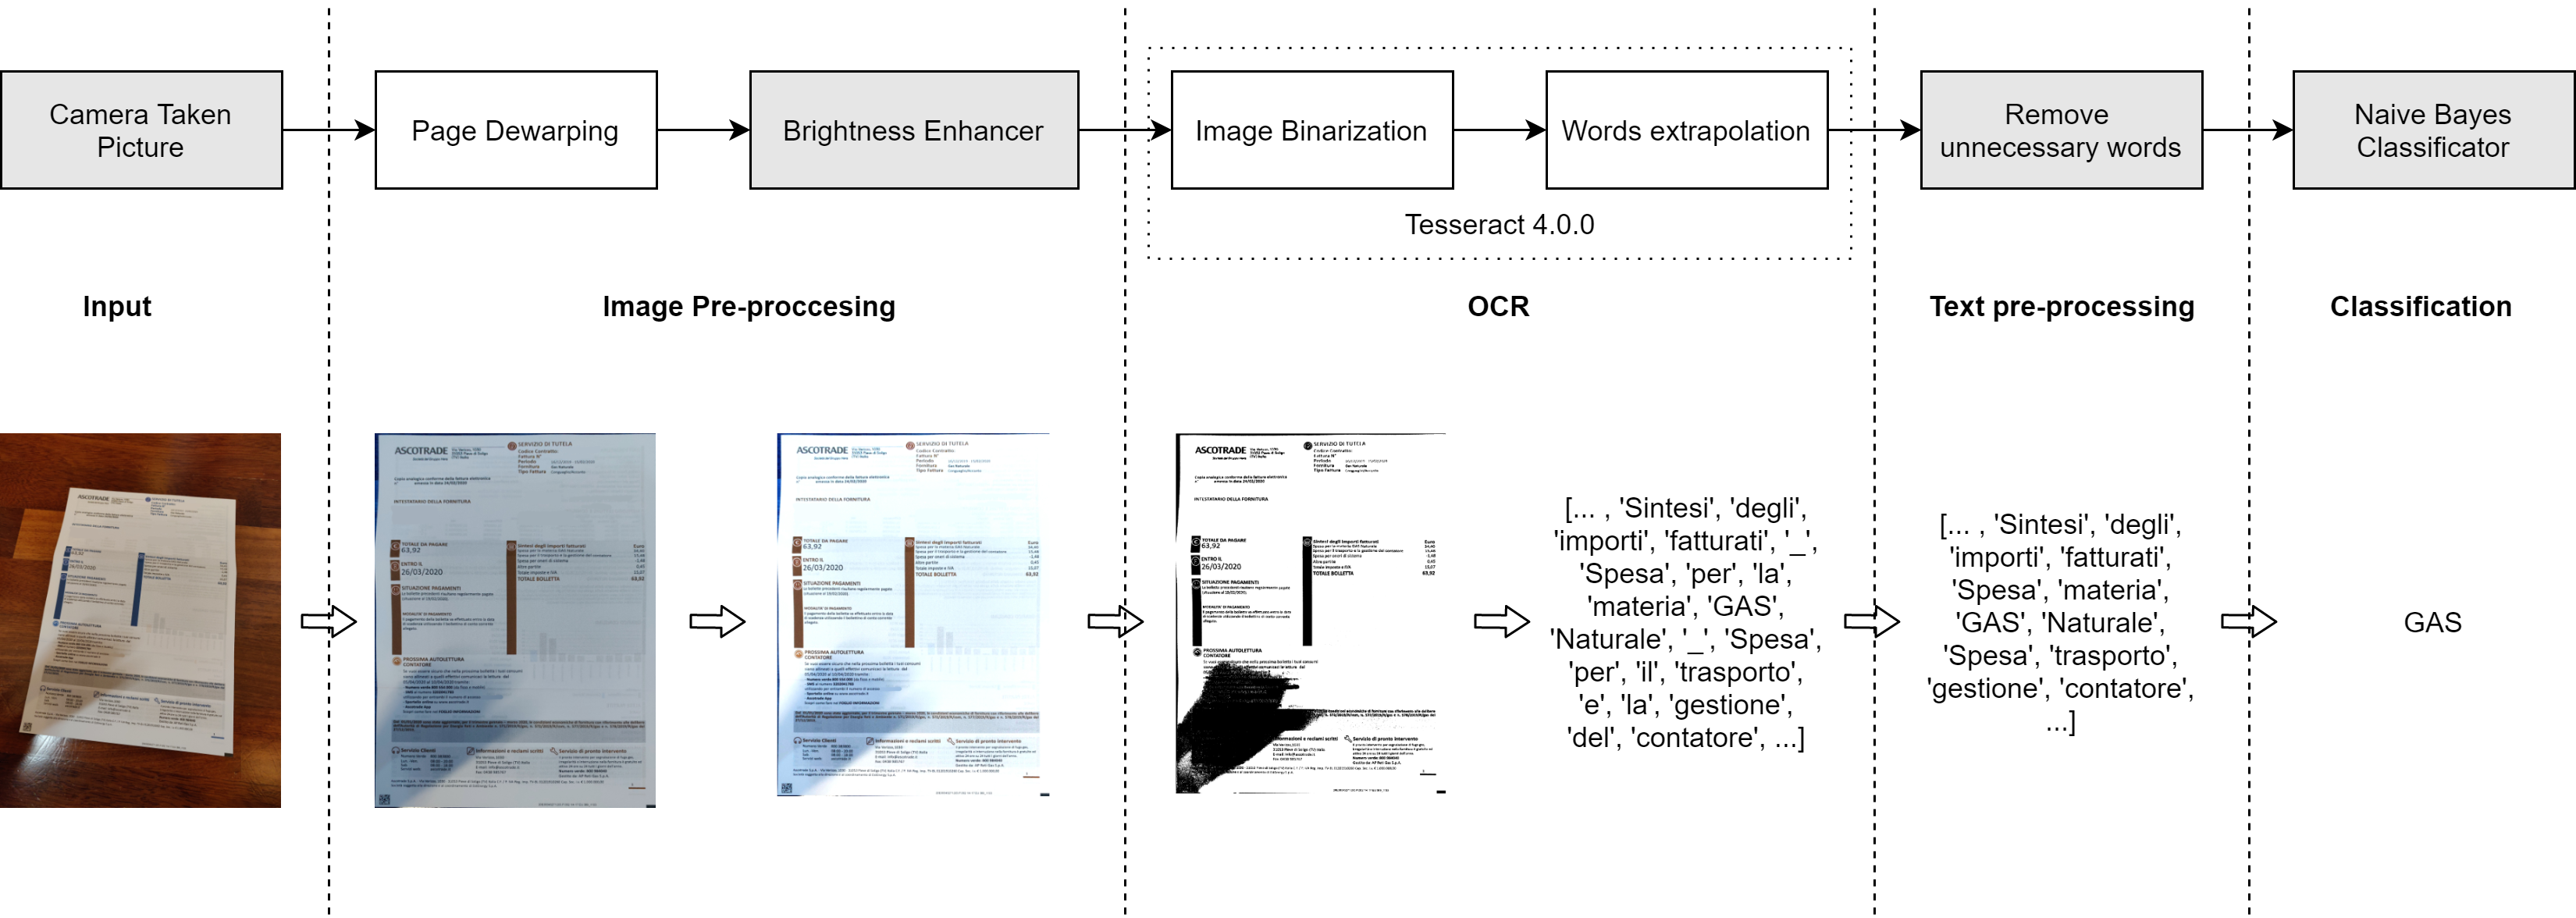
\includegraphics[width=1.0\textwidth]{images/pipeline.png}
	\caption{Our pipeline}
	\label{pipeline}
\end{figure*}

\subsection{Image pre-processing phase}
The image preprocessing phase is in charge of adjusting all the aspect of a mobile camera taken photos. This includes brightness and contrast adjustments, dewarping, skew correction and others. The first task of our pipeline infact is try to recover a flatbed scanned document from a camera taken photos. For this task we used the work done in \cite{mobile-ocr} wich uses an Xcenption Neural Network \cite{xception_NN} to perform this task, with appreciable results according to the article. In figure \ref{xception-architecture} is reported the Xception architecture used in this application coming from the work done in \cite{Improvingcamera-based}. We have seen that in some experiment, that involve the third dataset which consists of mobile camera taken in extreme conditions, the network doesn't correctly adjust the homography of the document. The last step of the image pre-processing is the correction of the brightness and constrast of the image. This is done because there are critical photos that could arise many problem for the OCR phase and this problems are be better exaplined in the Experiment section.

\subsubsection{The Xception Neural Network}
The dewarping phase is completly based on the work done in \cite{mobile-ocr}. Accordingly to the autor, the recovery of the homography of a mobile camera taken photos of a document is delegated to a Xception Neural Network. According to the paper \cite{xception} this architecture is based on Inception architecture wich first demonstrated the advantages of factoring the convolutions into multiple branches operating successively on channels and then on space. It uses then the Depthwise separable convolutions: unlike spatial separable convolutions (wich is used to reduce the computational complexity of a single convolution operation involving one kernel by dividing it into two smaller kernels), depthwise separable convolutions work with kernels that cannot be “factored” into two smaller kernels. The depthwise separable convolution is so named because it deals not just with the spatial dimensions, but with the depth dimension (the number of channels) as well. Similar to the spatial separable convolution, a depthwise separable convolution splits a kernel into 2 separate kernels that do two convolutions: the depthwise convolution and the pointwise convolution. We refer to this article \cite{https://towardsdatascience.com/a-basic-introduction-to-separable-convolutions-b99ec3102728} that exaplain better this two operation in the details with an example.\\

The used Xception neural network is trained over 1.5M synthetic images dataset. It uses Adam optimization method in combination with the L1-loss to predict the 4 corner points of the distorted document image. Then given this 4 obtained points from the Xception neurla network, the homography matrix H is computed by using Direct Linear Transforma (DLT). The network is made of 36 convolution layers and a total of 20,823,344 trainable parameter.

\begin{figure}[h]
	\centering
	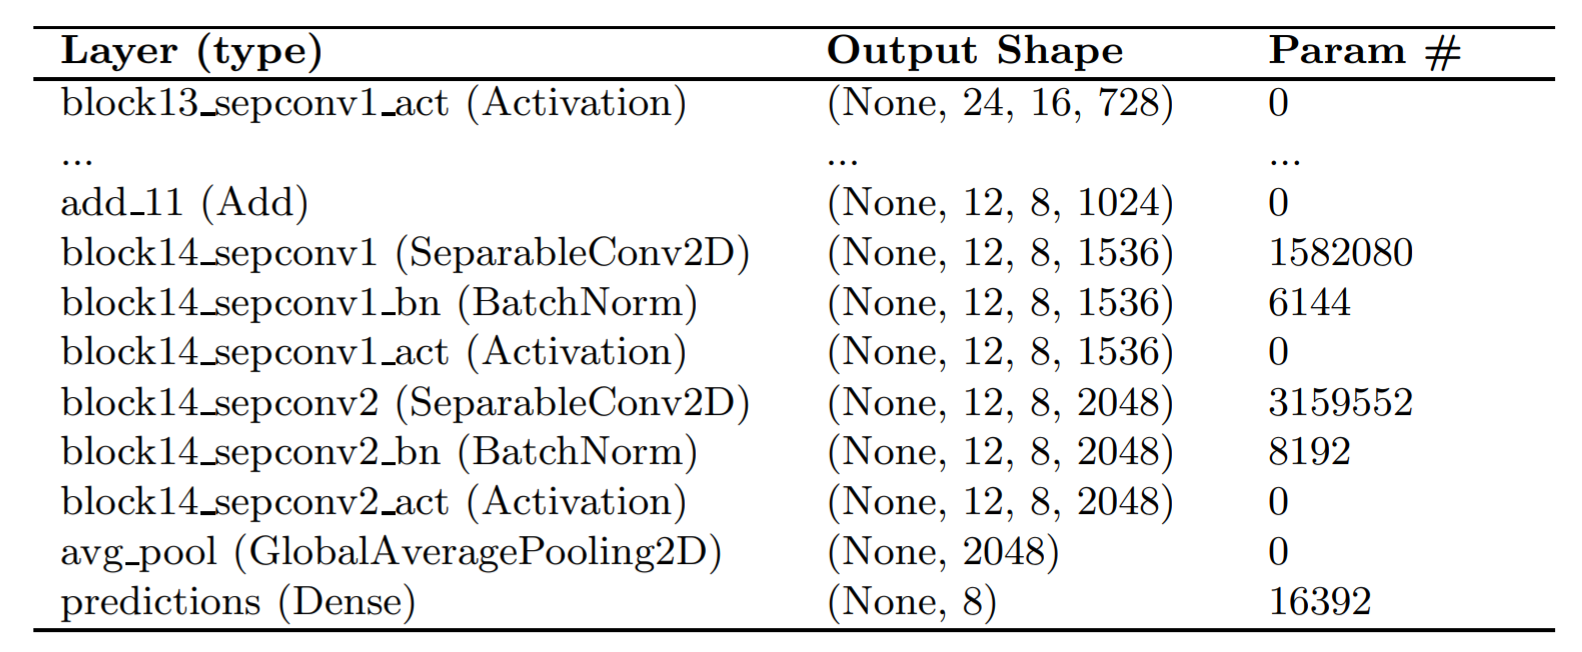
\includegraphics[width=0.48\textwidth]{images/xception-architecture.png}
	\caption{The Xception architecture used in this work}
	\label{xception-architecture}
\end{figure}

\subsection{OCR phase}
As we have seen this phase is delegated to Tesseract, which is a open-source OCR to extract all the words containded in a image. Tesseract is developed from Google and it is publically available on GitHub. 

\subsection{Text-preprocessing phase}
TODO

\subsection{Classification phase}
Speak about different classification alternatives like naive bayes, svm ecc ecc reported on different  articles TODO


\section{Experiments}

\subsection{Dewarping or not?}
As already widely discussed in the articles \cite{Improvingcamera-based} and \cite{recoveringhomography} the dewarping phase (also the deskew phase) is essential to improve the performance of Tesseract. We could confirm this fact with this experiment: we proccessed the same image, one time without dewarping it and the next time with the dewarping correction. If we highlight the extracted words in the two corresponding images we could see that there is a huge difference. Infact if we take a look at the figure \ref{dewarping-experiment} we could see that in the image without the dewarping correction the highlighted word are less than the same image dewarped and also the output is more precise and with fewer unneccesary random words that Tesseract could try to "guess". We could report that the extracted text for the non-dewarped image contains 708 words but a lot of them are blank spaces, while for the dewarped image the amout of extacted words are 491 but the output in this case is more precise and there are fewer blank spaces.

\begin{figure}[b]
	\centering
	\includegraphics[width=0.48\textwidth]{images/dewarping-experiment.png}
	\caption{Difference with and without dewarped text extraction}
	\label{dewarping-experiment}
\end{figure}


\subsection{Camera taken illuminance quality}
We have noticed during our expiremets that we have poor performances in the OCR phase if the mobile taken photos isn't correctly illuminated. Tesseract OCR, wich is the application designated for extracting the text of our bill in our application, already apply internally an image pre-processing step, trying to binarize the image for the later text extraction phase. The problem of this pre-processing step of Tesseract arise when the taken photos have a bad illumination or there are shadows present on it. Infact we could see in the example reported in figure \ref{bright-constrast-experiment} that if we take a poor illuminated photo of a bill and we print the pre-proccesing output of Tesseract we can noticed that there are completly white areas on the pre-processed photos and the binarization is inverted. For this reason if we try to increase the contrast and the brightness of the image we could see that the peformance are better. Infact if we take the same image as the example but this time we increase contrast and brightness we could notice that the pre-proccessed image of Tesseract is better, without too much area invisibles and also without the inversion of the binarization of the image. With this improvemets also the text extaction phase is more precise and accurate and it could extract all the words where before was contained in the white areas. For this reason we have inserted in the pipeline a "Brightness and Constrast Enhancer" for all the mobile taken photos (the jpg format), because we have seen that also if the image is already correctly illuminated and costrasted, even if we apply the enhancer, the performance are the same.

\begin{figure}[h]
	\centering
	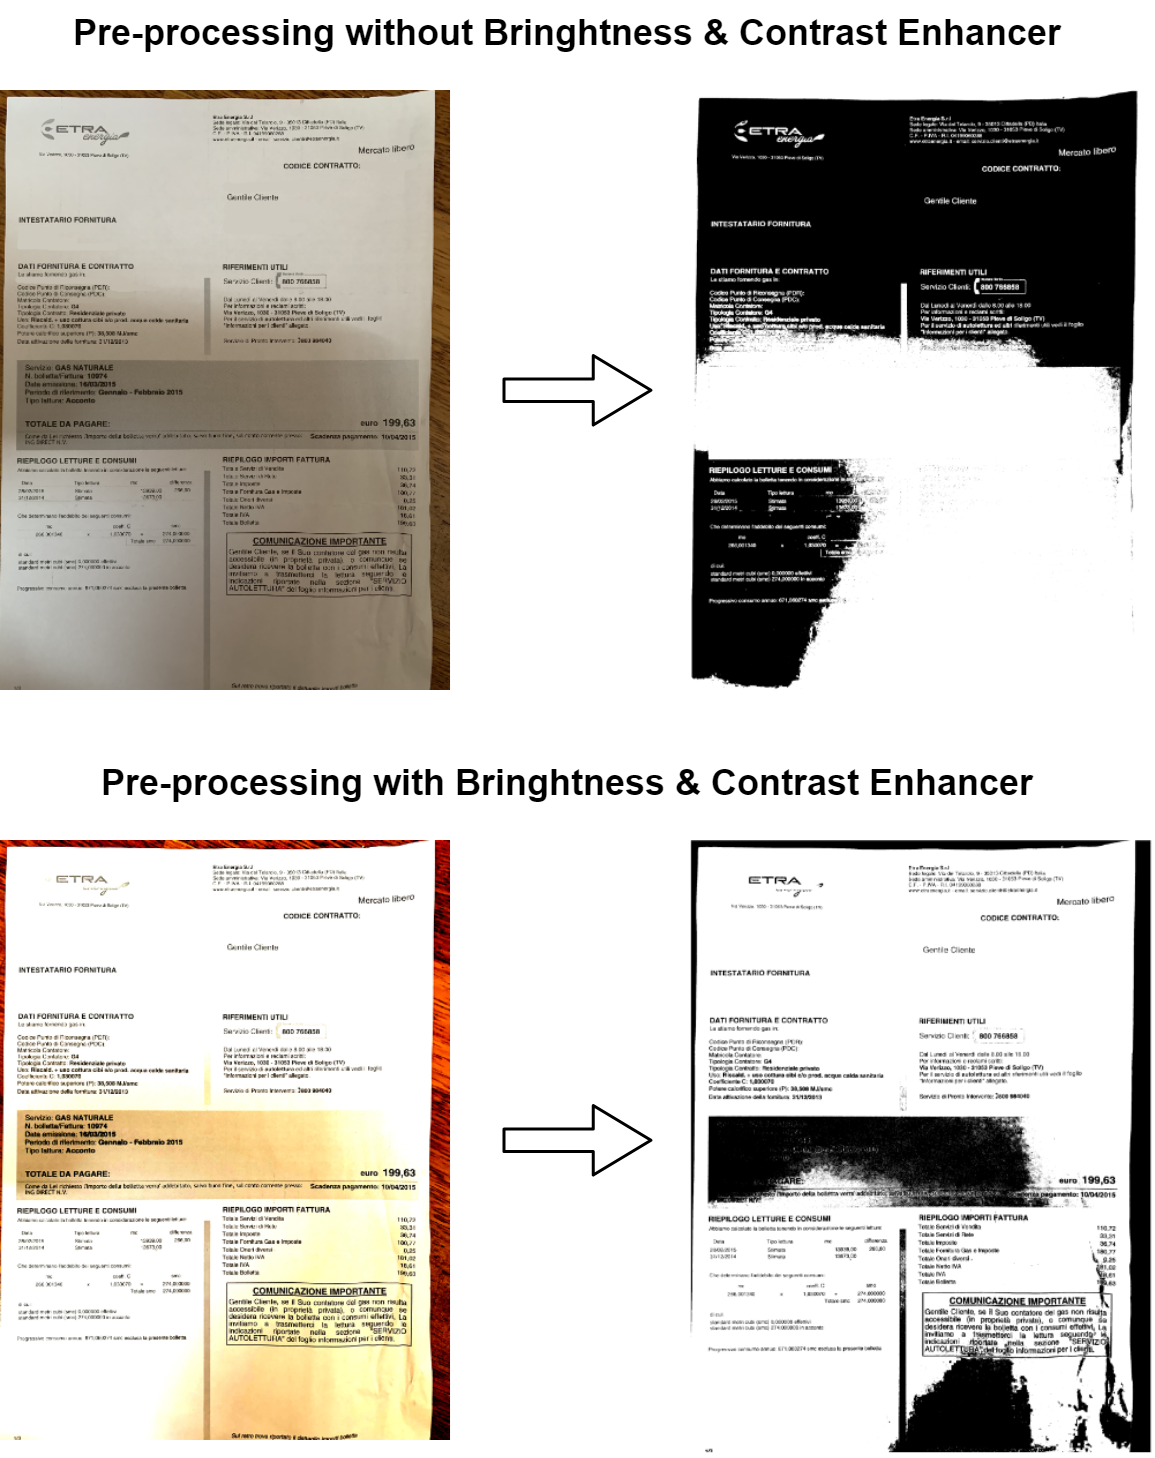
\includegraphics[width=0.4\textwidth]{images/bright-contrast-experiment.png}
	\caption{Difference with and without brightness and contrast enhancer}
	\label{bright-constrast-experiment}
\end{figure}


\subsection{Data augmentation}

\subsection{Machine Learning or Traditional Algorithms?}
Parlare del confronto tra un classificatore deterministico e un algorimo di machine learning, interessante sarebbec capire chi ha un accuratezza più alta. Confrontare anche con il numero di esempi richiesti.

\section{Conclusion}


{\small
\bibliographystyle{ieee_fullname}
\bibliography{egbib}
}

\end{document}
